\begin{frame}\frametitle{Sensor Fusion}%EKF implements sensor fusion. 
Sensor measurements are not available all the time - messages from sensors arrive at different moments and sensors could be unavailable due to different causes. 
\vspace{-5pt}
\begin{columns}
\column{.7\textwidth}
	\center{
    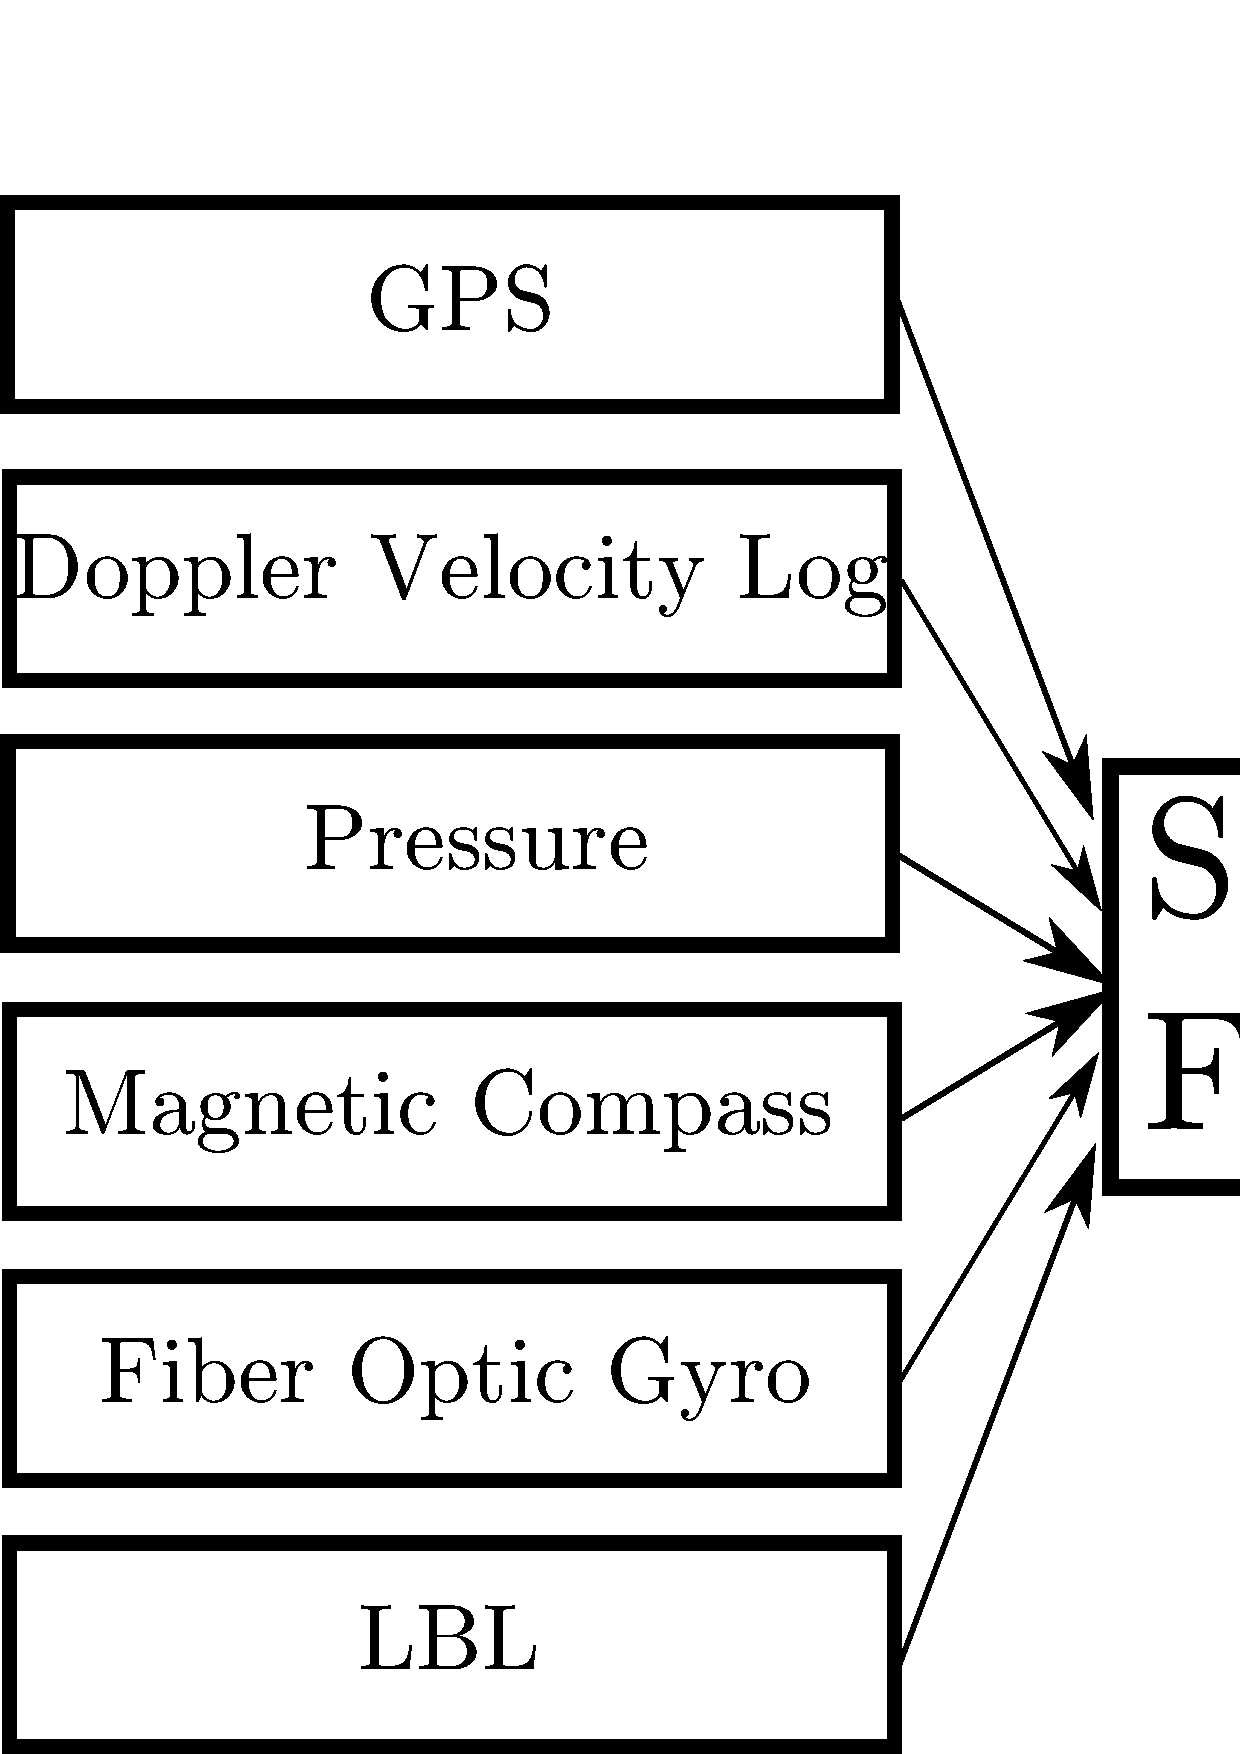
\includegraphics[width=0.98\linewidth]{fig/fusion-all.pdf}} \\
	\vspace{-5pt}
\hspace{3em} 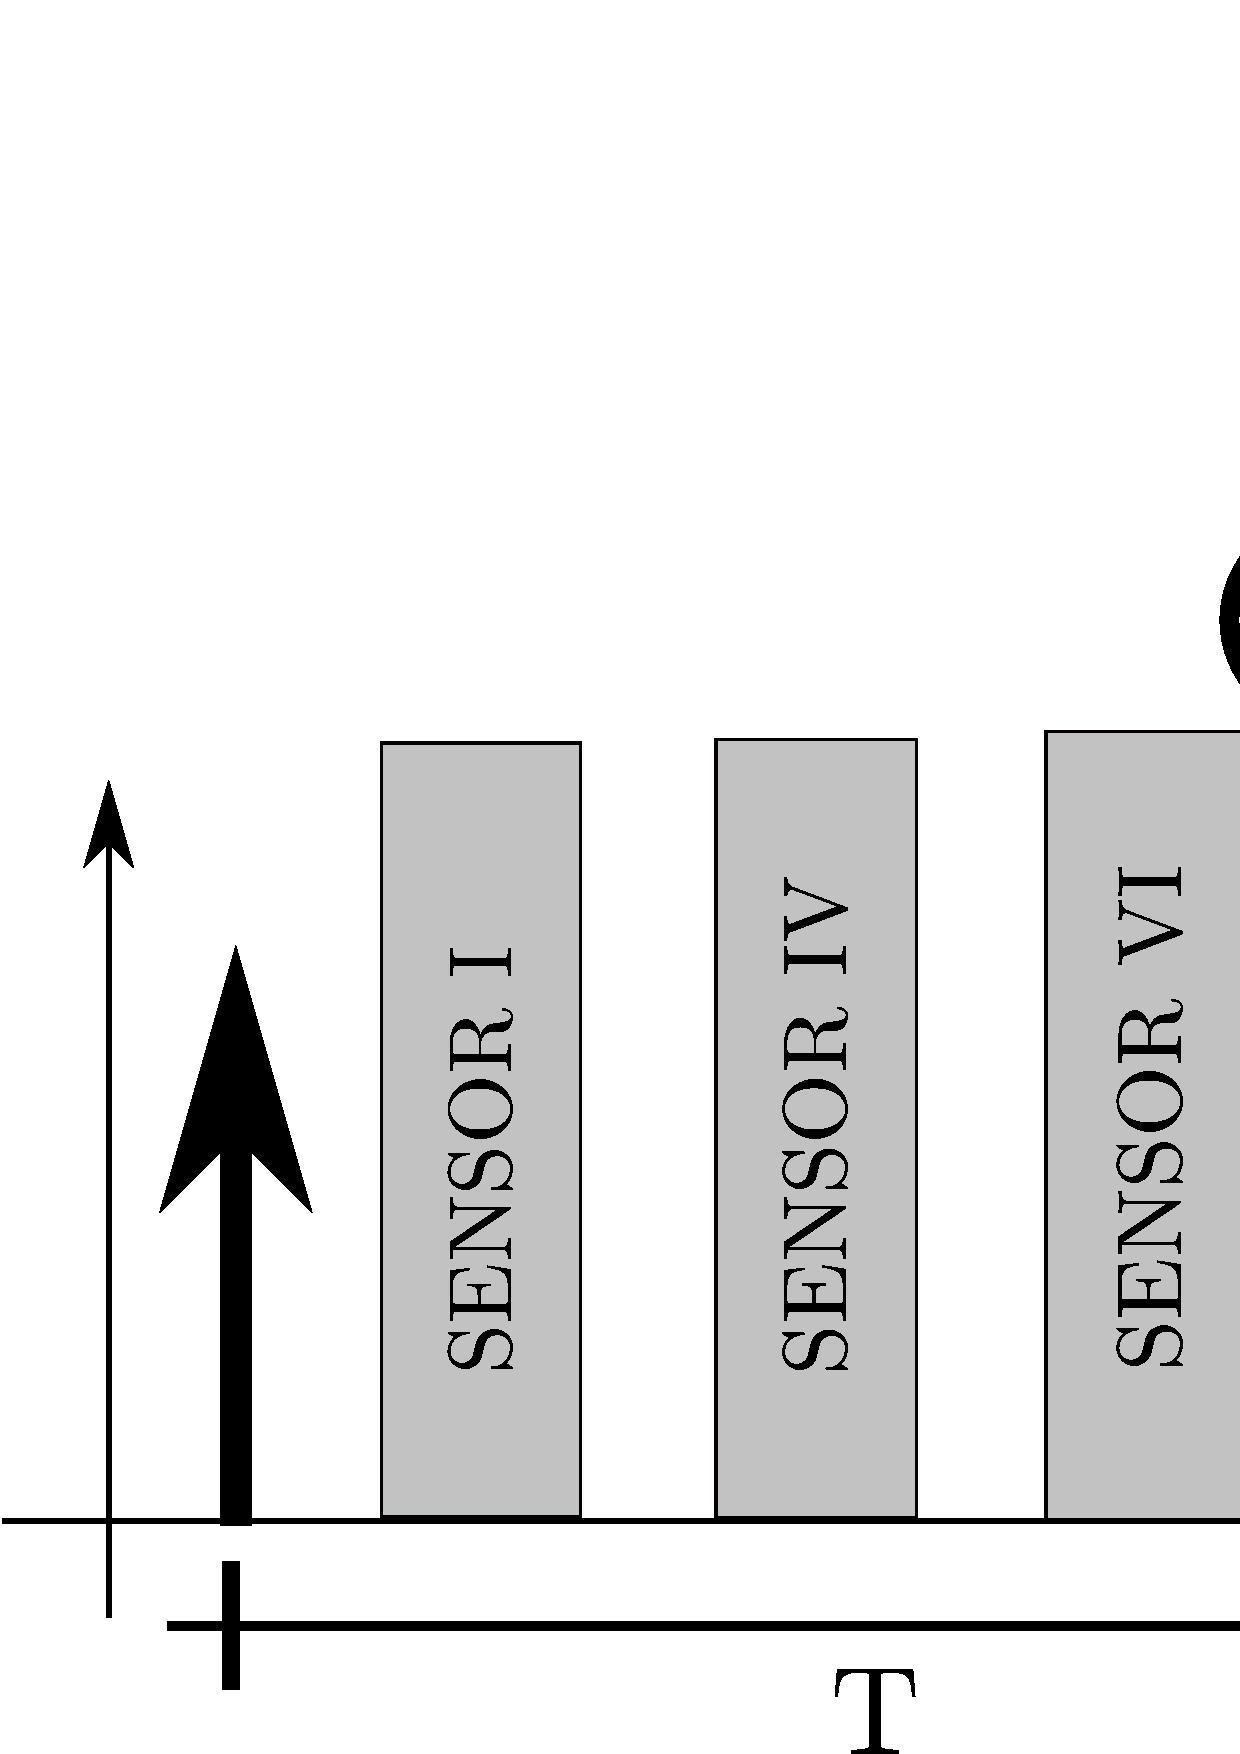
\includegraphics[width=0.43\linewidth]{fig/synch.pdf} 
\column{.28\textwidth}
	Gather the information in between the cycles and integrate it together in the measurement model (Eq. ~\ref{eq:fuse}).%, which varies depending on the measured values and sensors used for the measurement.
\end{columns}	
\begin{equation}
\label{eq:fuse}
\vect{Z}(k) = \left[ \begin{array}{c} \vect{Z}_{sen. I} \\ \vect{Z}_{sen. II}  \end{array} \right],
\vect{H}(k) = \left[ \begin{array}{c} \vect{H}_{sen. I} \\ \vect{H}_{sen. II}  \end{array} \right], 
\vect{R}(k) = \left[ \begin{array}{cc} \vect{R}_{sen. I} & 0 \\ 0 & \vect{R}_{sen. II} \end{array} \right]
\end{equation}
\vspace{-10pt}	
	\begin{equation*}
	\vect{Z}(k) = h(\vect{X}(k), \vect{M}(k)) = \vect{H} \vect{X}(k \mid k-1)  + \vect{M}(k)
	\end{equation*}
%parameters 
$\vect{R}_{sen. I}$ and $\vect{R}_{sen. II}$ are defining sensor measurement (un)certainty.
\end{frame}